% ---------------------------- Preamble starts here ----------------------------

\documentclass[aspectratio=169]{beamer} %Remove [aspectratio=169] to get non-wide 4:3 slide aspect ratio

%-----------------------------------------------
% --- Set beamer theme
\usetheme{Metropolis}
\setbeamertemplate{footline}{}				% Remove automatic footer
\setbeamertemplate{navigation symbols}{}	% Comment this line to display navigation symbols

%-----------------------------------------------
% Load i2i symbol
\addtobeamertemplate{frametitle}{}{%
\begin{textblock*}{\linewidth}(0cm,7.1cm) % Replace with (0cm, 8cm) if using non-wide slide aspect
	
\includegraphics[width=\linewidth]{../../Common-Resources/img/Footer.png}
\end{textblock*}}

%-----------------------------------------------
% --- Load packages
\usepackage{textpos}		% To align objects correctly
\usepackage{multicol}		% To right in multiple columns
\usepackage{color}			% To color text

%-----------------------------------------------
% --- Include link to last commit
\usepackage{xstring}
\usepackage{catchfile}

%Set this user input
\newcommand{\gitfolder}{../../../.git} %relative path to .git folder from .tex doc
\newcommand{\reponame}{worldbank/dime-github-trainings} % Name of account and repo be set in URL

%Based on this https://tex.stackexchange.com/questions/455396/how-to-include-the-current-git-commit-id-and-branch-in-my-document
\CatchFileDef{\headfull}{\gitfolder/HEAD.}{} 				%Get path to head file for checked out branch
\StrGobbleRight{\headfull}{1}[\head]						%Remove end of line character
\StrBehind[2]{\head}{/}[\branch]							%Parse out the path only
\CatchFileDef{\commit}{\gitfolder/refs/heads/\branch.}{}	%Get the content of the branch head
\StrGobbleRight{\commit}{1}[\commithash]					%Remove end of line characted

%Build the URL to this commit based on the information we now have
\newcommand{\commiturl}{\url{https://github.com/\reponame/commit/\commithash}}

%-----------------------------------------------
% --- Add your information here
\title{An intro to Git and GitHub - Team Maintainer}
\author{DIME Analytics}
\institute{DIME - The World Bank - \trainingURL{https://www.worldbank.org/en/research/dime}}
\date{\today}

\newcommand{\trainingURL}[1]{{\color{blue}\url{#1}}}

\newcommand{\traininerUsername}{kbjarkefur}
\newcommand{\repoName}{\traininerUsername/lyrics-Jun17}
\newcommand{\trainingRepoURL}[1]{\trainingURL{github.com/\repoName #1}}
\newcommand{\trainerEmail}{\trainingURL{kbjarkefur@worldbank.org} }


% ---------------------------- Preamble ends here ----------------------------

\begin{document}

\begin{frame}

\includegraphics[width=\textwidth]{../../Common-Resources/img/Header.png}
\vspace{-0.2cm}
\titlepage 	 % Opening slide, prints inform
\end{frame}

\begin{frame}
\frametitle{Objectives}

This is the topics that we will cover in this training:
	\begin{itemize}
		\item Why do we bother with teams?
		\item Quick guide to how to do team maintainer tasks
		\item What other tasks do we ask the team maintainers to help us with?
	\end{itemize}
\end{frame}


\begin{frame}
	\frametitle{Quick role overview}
	
	\begin{columns}[T]
		
		\column{.15\textwidth} % Left buffer
		
		\column{.30\textwidth} % Left column and width
		\textbf{Repo roles:}
		\begin{itemize}
			\item Contributor
			\item Repo Maintainer
			\item Repo Admin
		\end{itemize}
	
		\column{.10\textwidth} % Middle buffer
		
		\column{.30\textwidth} % Right column and width
		\textbf{Team roles:}
		\begin{itemize}
			\item Member
			\item Team Maintainer
		\end{itemize}	
	
		\column{.15\textwidth} % Right buffer
		
	\end{columns}
\end{frame}


%%%%%%%%%%%%%%%%%%%%%%%%%%%%%%%%%%%%%%%%%%%%%%%%%%%%%%%%%
%% Why bither with teams?

\section{Overview and work flow}

\begin{frame}
	\frametitle{Objectives}
	
	\begin{itemize}
		\item As default we do not give the project teams admin access to the repos
		
		\item With admin access you can do potentially destructive actions -- such as deleting the whole repo and all its history. 
		
		\item We still want you to give access to the teams to add and remove users from the repo without having to ask DIME Analytics each time.
		
		\item On GitHub, Teams can be used to control access to repos without giving admin access

	\end{itemize}
\end{frame}

\begin{frame}
	\frametitle{GitHub Teams Creation Work Flow}

	\begin{columns}[c]
		
		\column{.60\textwidth} % Left column and width
		\begin{enumerate}
			\item DIME Analytics creates a team
			\item DIME Analytics makes one team member the \textit{team maintainer}
			\item DIME Analytics creates a repo and adds the team to the repository
			\item The team maintainer add and remove user to the team to grant and revoke access to the repo
			\item Only users added to the DIME organization account can be added to teams
		\end{enumerate}
		
		\column{.40\textwidth} % Right column and width
		\begin{figure}
			\centering
			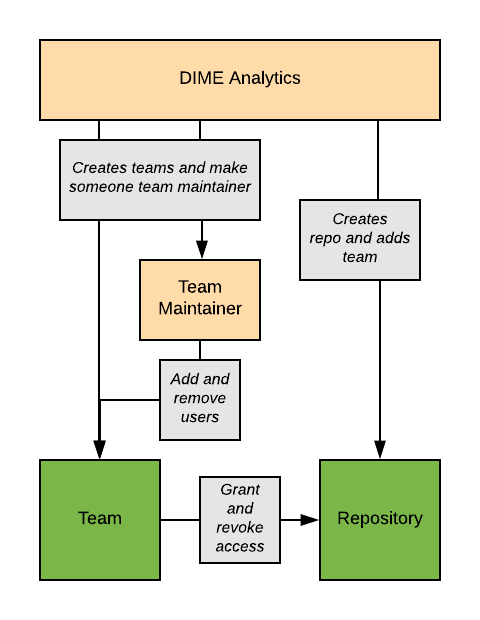
\includegraphics[width=1\linewidth]{./img/teams-workflow}
		\end{figure}
		
	\end{columns}
\end{frame}


\begin{frame}
	\frametitle{Quick talking points}
	
	\begin{columns}[c]
		
		\column{.50\textwidth} % Left column and width
		Quick facts about teams:
		\begin{itemize}
			\item There can be more than one team maintainer for a team
			\item A team can be used for more than one repo
			\item A repo can have more than one team added to it
		\end{itemize}
		
		\column{.50\textwidth} % Right column and width
		Admin access vs. Teams
		\begin{itemize}
			\item Can I be made admin instead of dealing with teams?
			\item Sure, but we will ask for the TTL's approval to do so after explaining to them the risks associated with admin access
		\end{itemize}	
		
	\end{columns}
\end{frame}

%%%%%%%%%%%%%%%%%%%%%%%%%%%%%%%%%%%%%%%%%%%%%%%%%%%%%%%%%
%% Quick overview how to do things 

\section{How to do Team actions on GitHub.com}

\begin{frame}
	\frametitle{Which teams am I in?}
	\textbf{How do I know which teams I am in?}
	\begin{enumerate}
		\item Go to \url{https://github.com/dime-worldbank} and click \textit{Teams}
		\item Then search for your username, like \textit{@username}
	\end{enumerate}
	\centering
	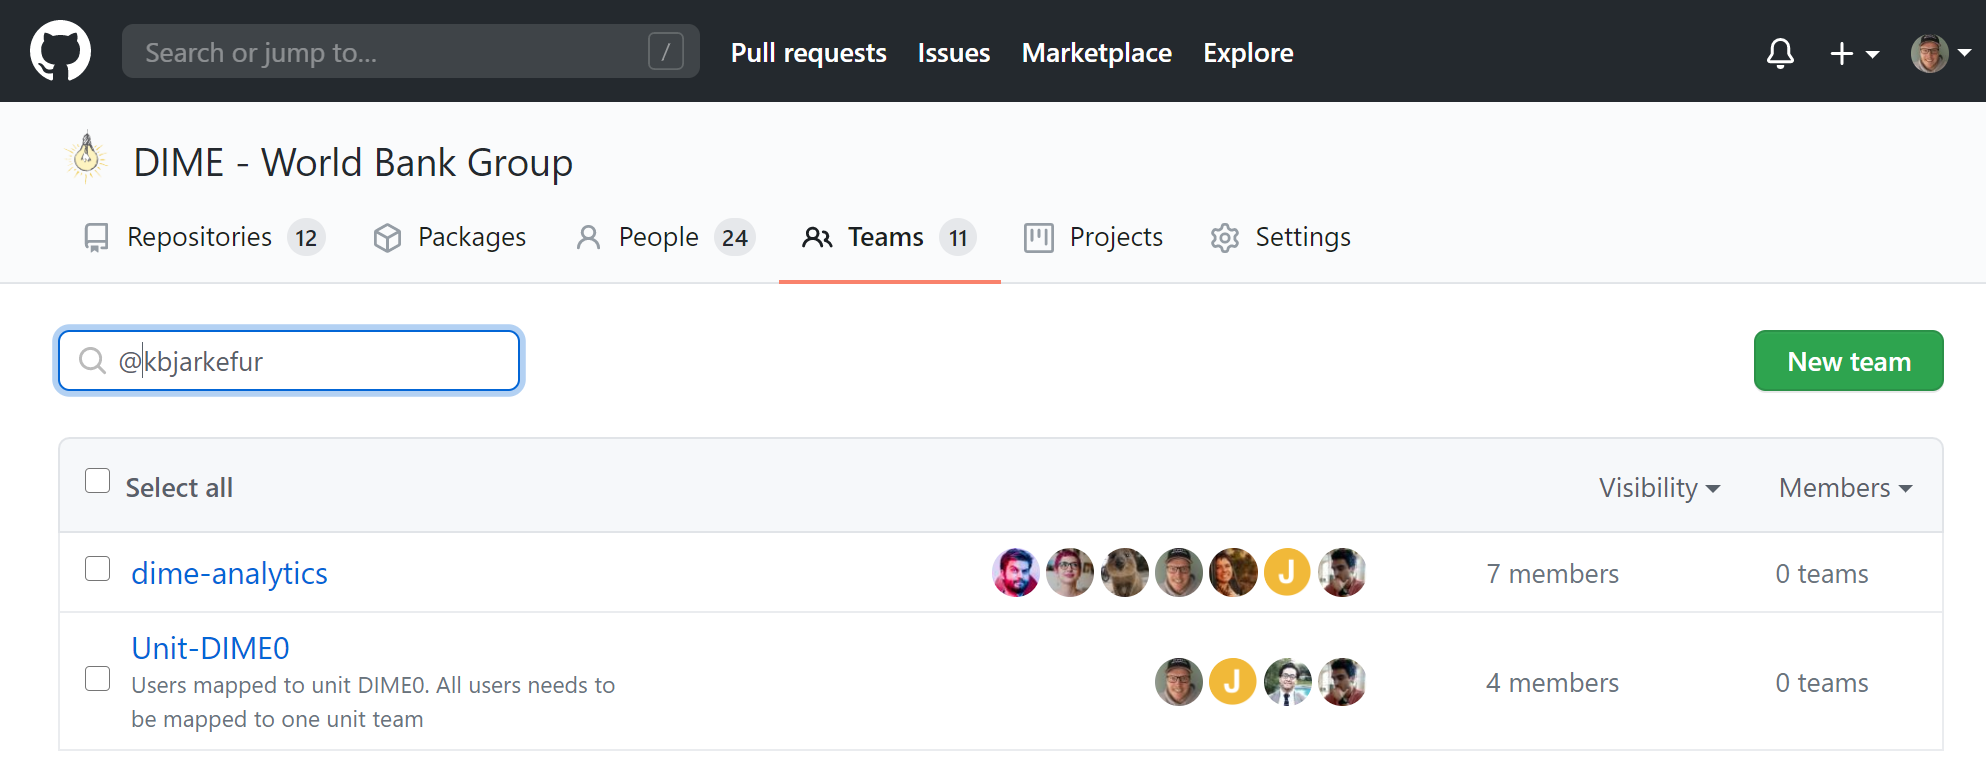
\includegraphics[width=.8\linewidth]{./img/which-teams-am-i-in}
\end{frame}


\begin{frame}
	\frametitle{Am I a team maintainer for a team?}
	\begin{columns}[c]
		
		\column{.30\textwidth} % Left column and width
		\textbf{Check who is team maintainer:}
		\begin{enumerate}
			\item Click the team name
			\item Click \textit{Members}
			\item See who has the \textit{Maintainer} sticker
		\end{enumerate}
		
		\column{.70\textwidth} % Right column and width
		\begin{figure}
			\centering
			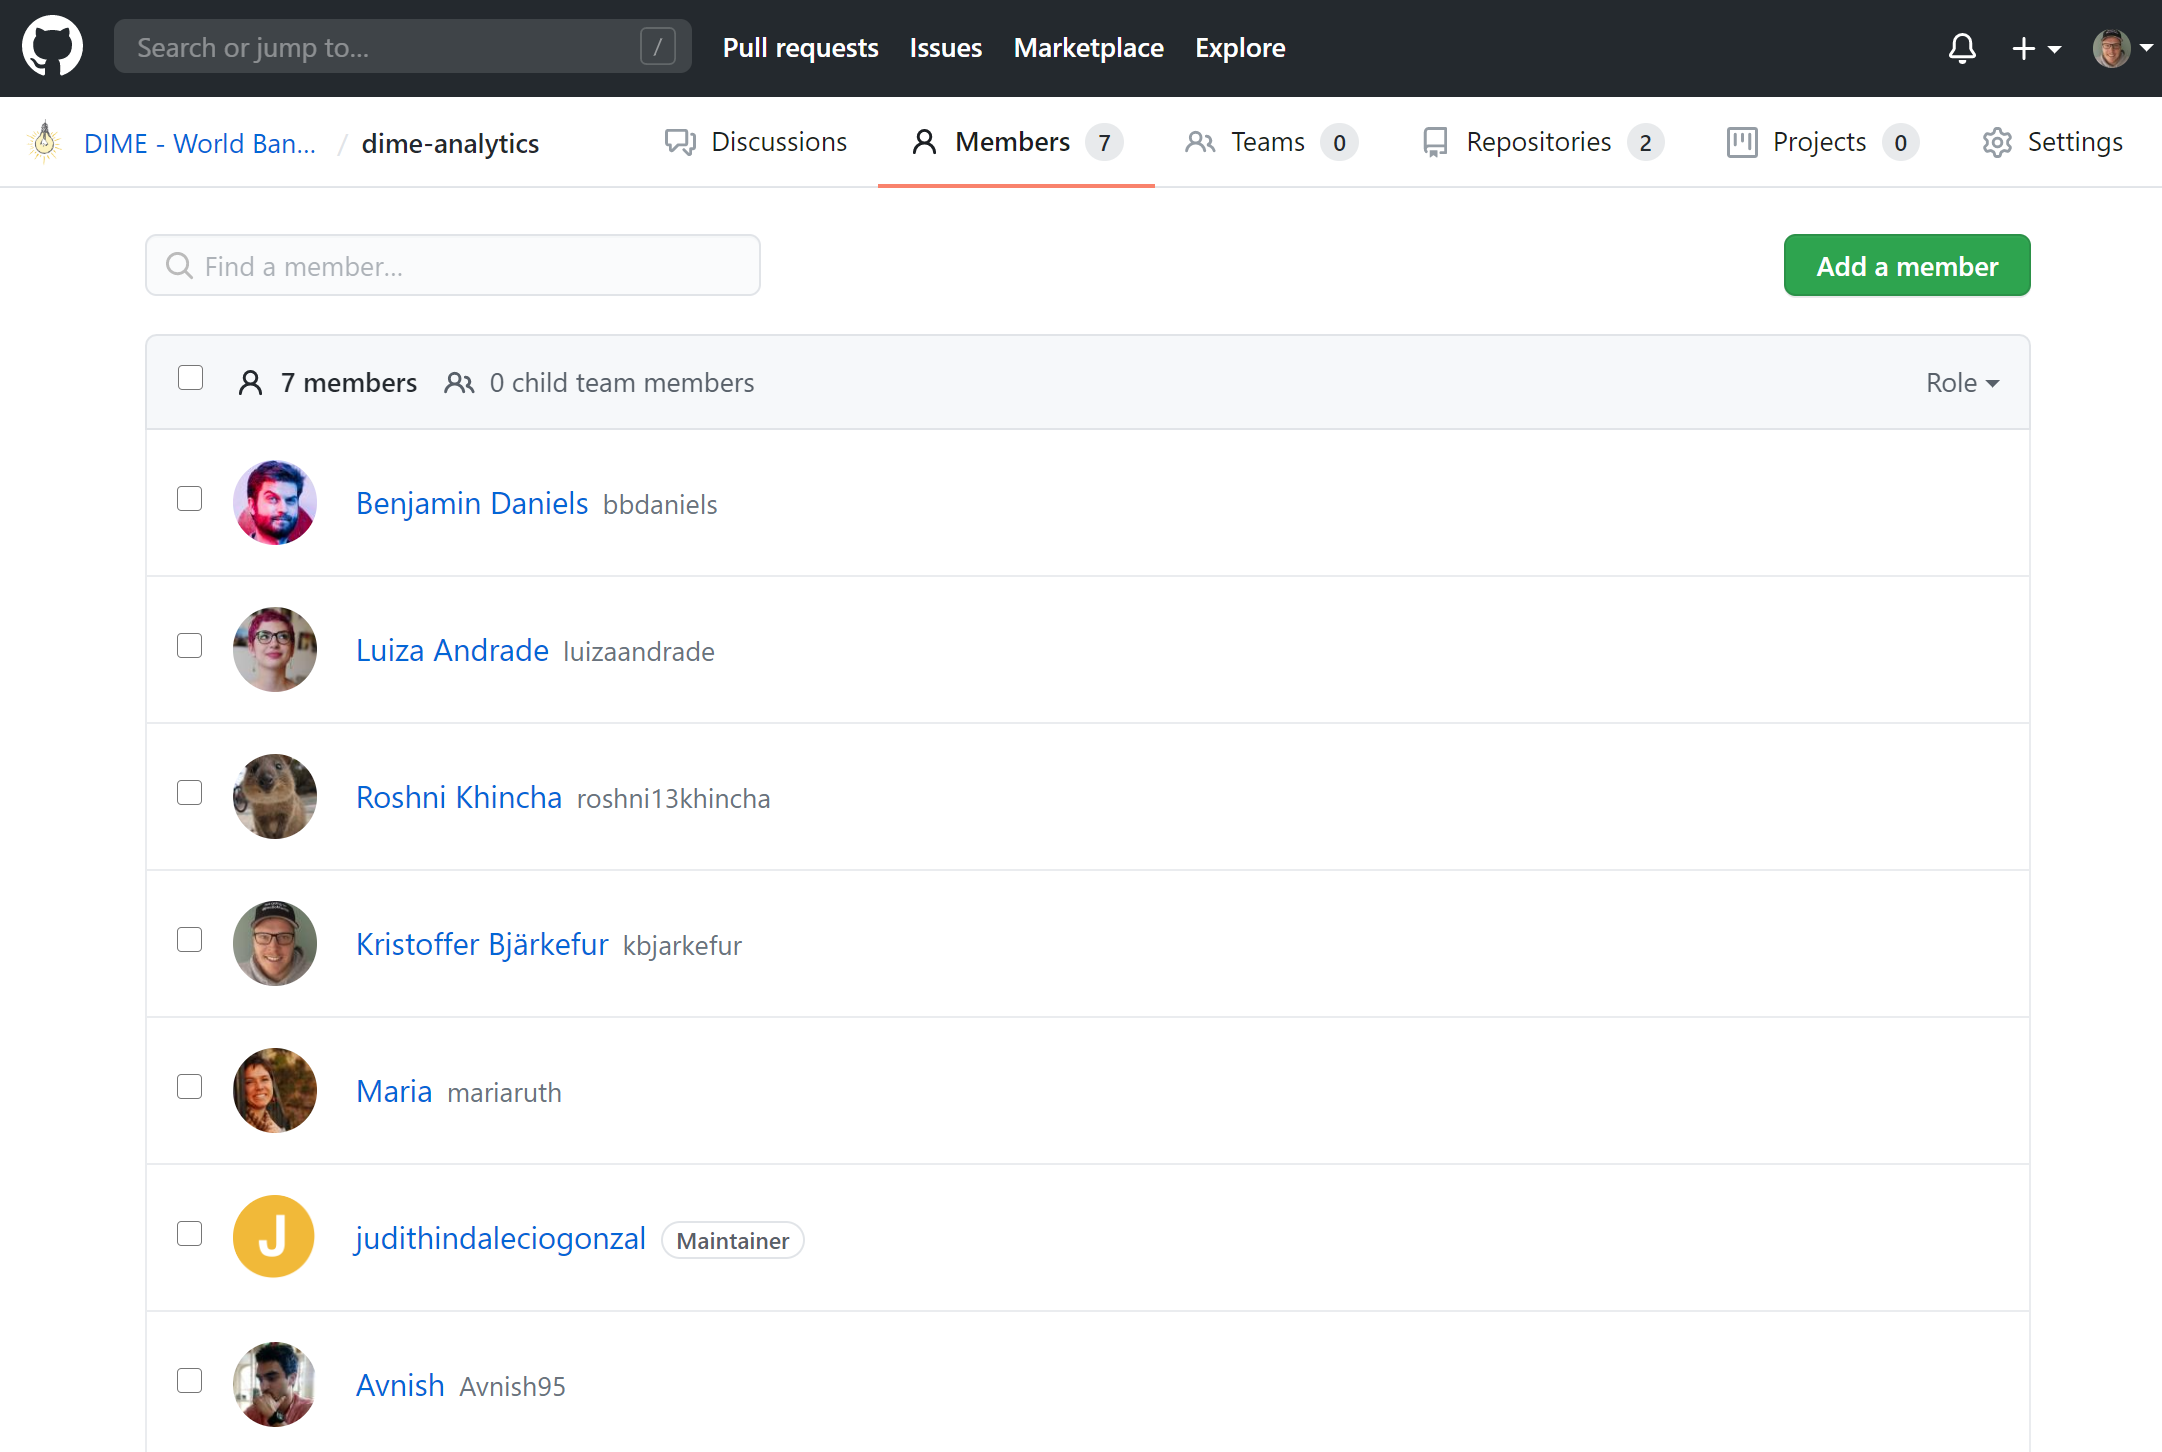
\includegraphics[width=1\linewidth]{./img/who-is-team-maintainer}
		\end{figure}
	\end{columns}
\end{frame}


\begin{frame}
	\frametitle{How do I manage team members?}
	\begin{columns}[c]
		
		\column{.30\textwidth} % Left column and width
		\textbf{Add user:}
		\begin{enumerate}
			\item Click \textit{Add a member}
			\item Enter new members username
		\end{enumerate}

		\textbf{Remove user:}
		\begin{enumerate}
			\item Check the check box next to user
			\item Select \textit{Remove from team} in the menu that appears above the list of memebers
		\end{enumerate}


		\column{.70\textwidth} % Right column and width
		\begin{figure}
			\centering
			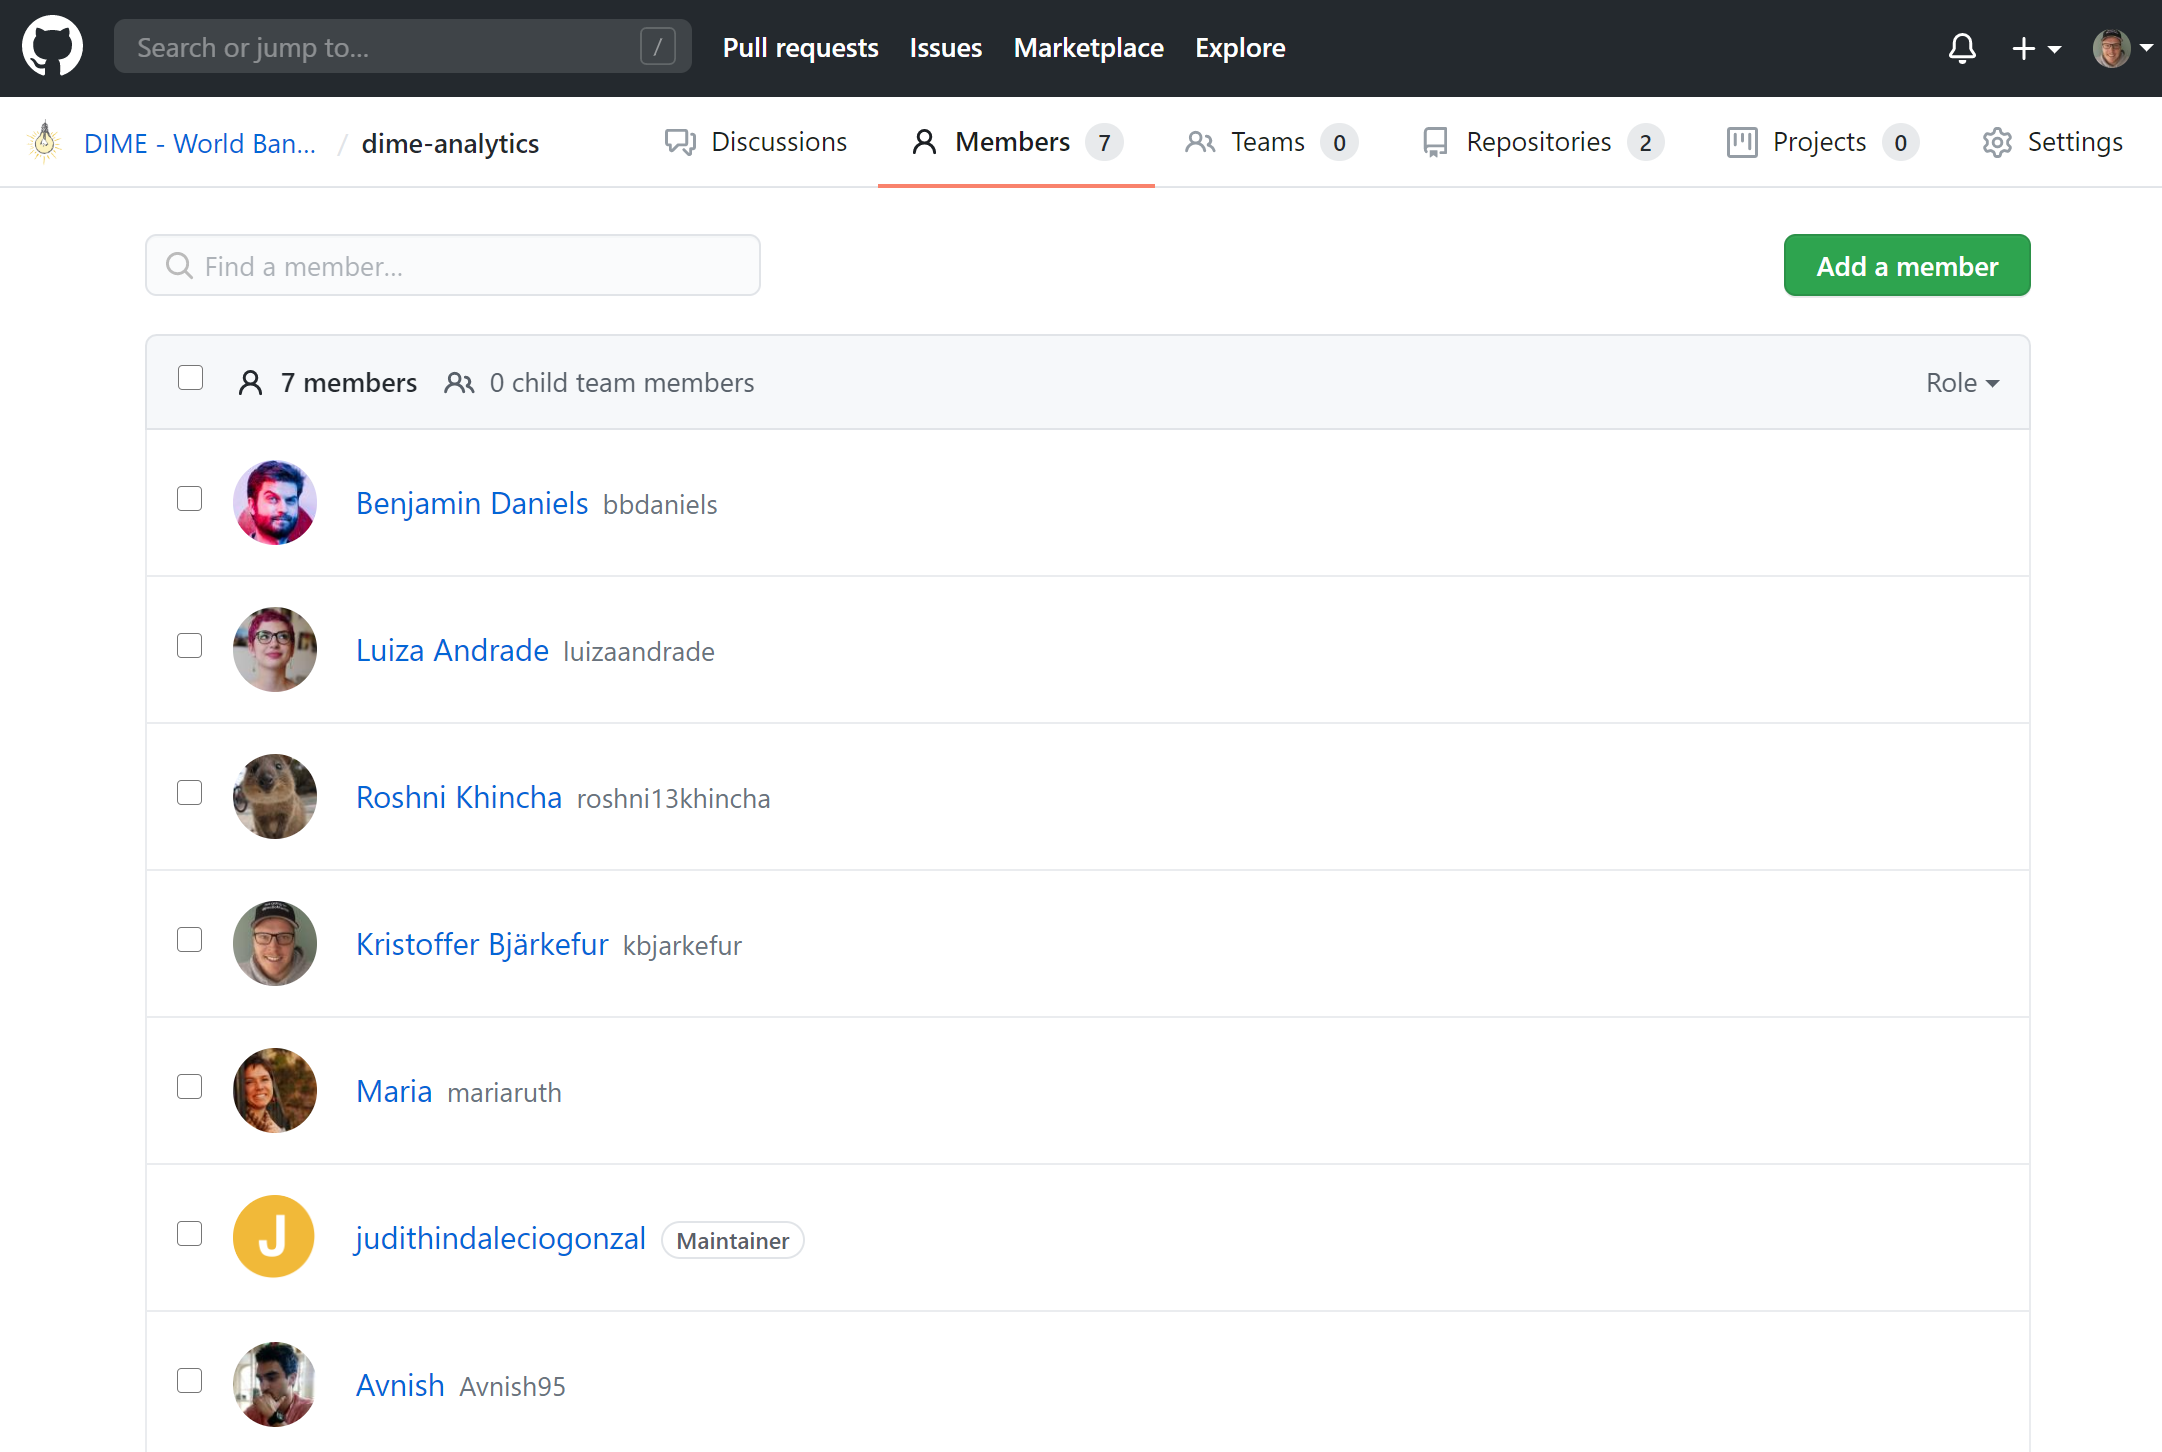
\includegraphics[width=1\linewidth]{./img/who-is-team-maintainer}
		\end{figure}
	\end{columns}
\end{frame}


\begin{frame}
	\frametitle{Which repos is a team used for?}
	\textbf{Which repos are a team used for?}
	\begin{enumerate}
		\item In the team page, click \textit{Repositories}
	\end{enumerate}
	\centering
	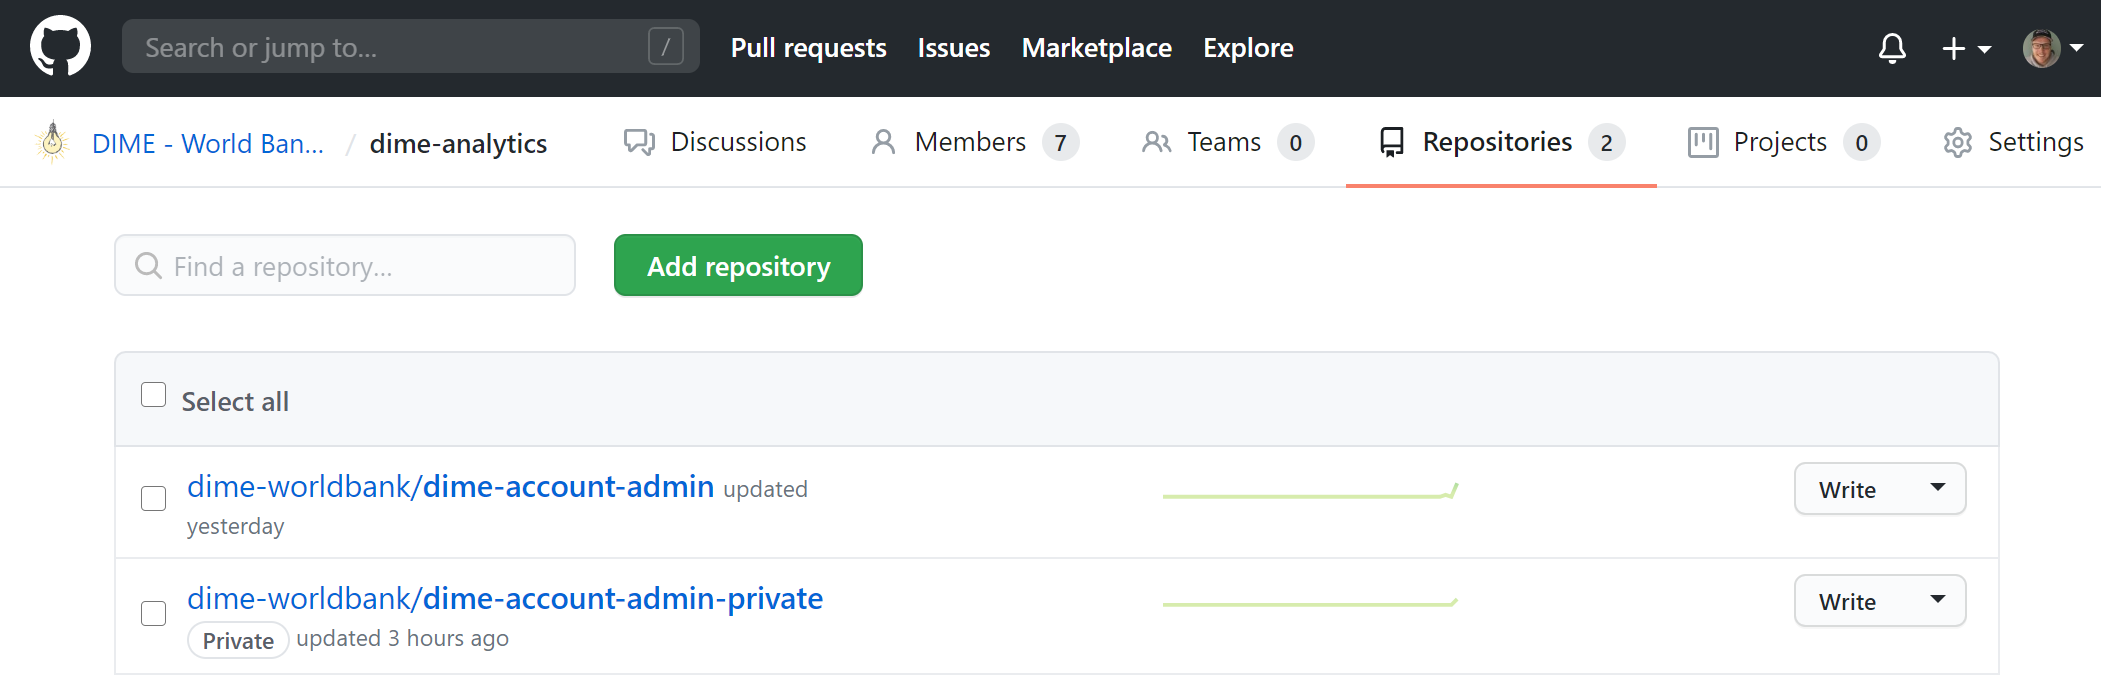
\includegraphics[width=.8\linewidth]{./img/which-repos-in-team}
\end{frame}


\begin{frame}
	\frametitle{Which teams are used for a repo?}
	\begin{columns}[c]
		\column{.30\textwidth} % Left column and width
		\textbf{Which teams in used in a repo?}
		\begin{enumerate}
			\item Go to \url{https://github.com/worldbank/dime-github-admin}
			\item Click reports, then click your repo
			\item Scroll down to collaborators and check the columns
		\end{enumerate}
		
		\column{.70\textwidth} % Right column and width
		\begin{figure}
			\centering
			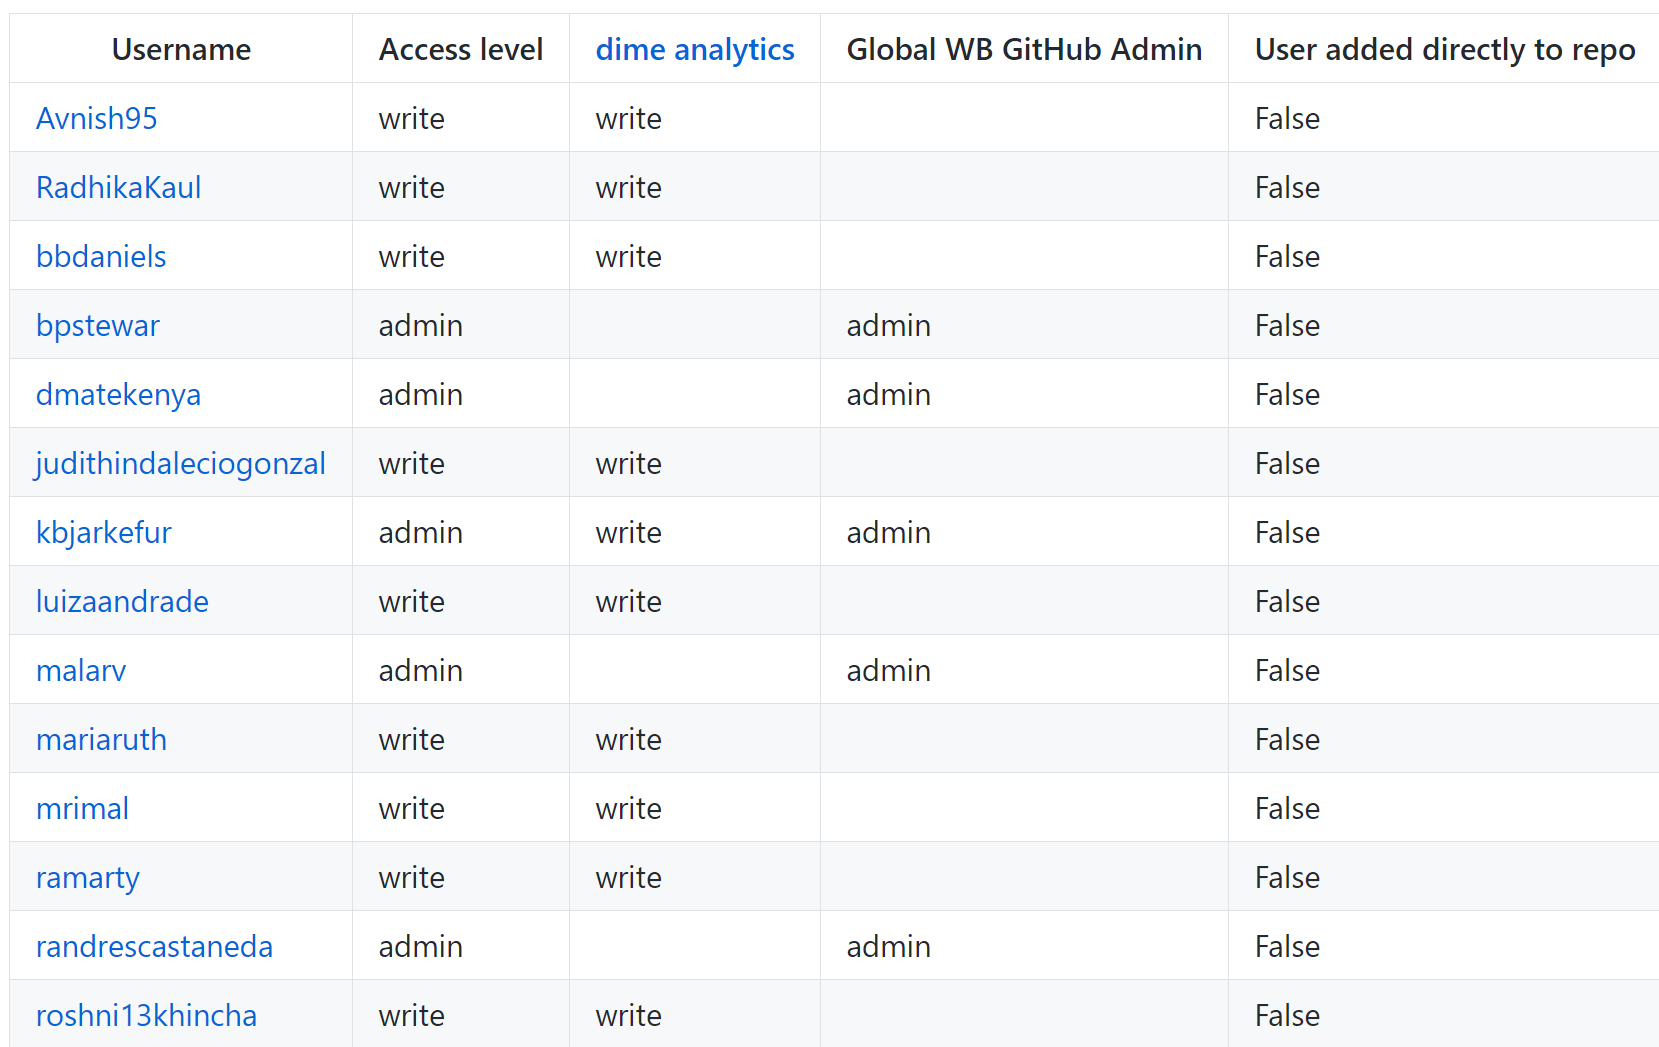
\includegraphics[width=1\linewidth]{./img/which-teams-in-repo}
		\end{figure}
	\end{columns}		
\end{frame}


%%%%%%%%%%%%%%%%%%%%%%%%%%%%%%%%%%%%%%%%%%%%%%%%%%%%%%%%%
%% Other tasks

\section{Other tasks involving team maintainers}

\begin{frame}
	\frametitle{Other tasks involving team maintainers}
	
	\begin{itemize}
		\item We will use the team maintainer as the contact person for repos linked to a team
		
		\item If admins have a question about a repo, then we will contact the team maintainer/maintainers for the team/teams linked to that repo. The team maintainer does not need to know all answers, but should at least know who to talk to 
		
		\item Whenever admins are performing a large scale process, such as a transfer, we will turn to team maintainers for help

	\end{itemize}
\end{frame}

%%%%%%%%%%%%%%%%%%%%%%%%%%%%%%%%%%%%%%%%%%%%%%%%%%%%%%%%%
%% Transfer 

\section{Transfer to dime-worldbank account}

\begin{frame}
	\frametitle{dime-worldbank account set up}
	
	\begin{itemize}
		\item In the new account we have an unlimited number of private and public repositories, but instead we pay for users.
		\item We pay for all users added to the the organization account.
		\item We pay for external collaborators added private repositories, but not for public repositories.
		\item DIME Analytics covers this cost for the foreseeable future, in return we just ask the team maintainers to help us remove people as they leave.
	\end{itemize}
\end{frame}


\begin{frame}
	\frametitle{Team maintainers tasks on transfer}
	
	\begin{enumerate}
		\item Check that all team members are still current members
		\item Check that all external collaborators for all repos the team is used for are still current users
		\item Decide if public repos should be transferred or not
		\item Help us communicate to the team. We provide a template for that communication, but it is better if it comes from you
	\end{enumerate}

	 If you are interested, see our full transfer protocol here: \url{https://github.com/dime-worldbank/dime-account-admin-private/blob/master/transfer-from-old-account/README.md}
\end{frame}

%%%%%%%%%%%%%%%%%%%%%%%%%%%%%%%%%%%%%%%%%%%%%%%%%%%%%%%%%
%% Discussion

\section{Discussion}

\begin{frame}
	\frametitle{Discuss best practices}
	
	\begin{itemize}
		\item Big teams for many repos or one small team per repo?
		\item A team maintainer should know of the repos a team is used for but does not need to work on the projects for those repos
		\item Multiple team maintainer in one team?
		\item Give admin access to the research team?
		\item Other questions to discuss?
	\end{itemize}
	
\end{frame}

%%%%%%%%%%%%%%%%%%%%%%%%%%%%%%%%%%%%%%%%%%%%%%%%%%%%%%%%%
%% End boiler plate

\section{Links}

\begin{frame}{Useful links}
	\begin{itemize}
	  \item All DIME Analytics GitHub resources: \trainingURL{https://github.com/worldbank/dime-github-trainings}. For example:
		\begin{itemize}
			\item DIME Analytics GitHub Templates (for example .gitignore): \trainingURL{https://github.com/worldbank/dime-github-trainings/tree/master/GitHub-resources/DIME-GitHub-Templates}
			\item DIME Analytics GitHub Roles: \trainingURL{https://github.com/worldbank/dime-github-trainings/blob/master/GitHub-resources/DIME-GitHub-Roles/DIME-GitHub-roles.md}
		\end{itemize}
		\item Markdown cheat sheet (how to format text on GitHub.com):  \trainingURL{https://www.markdownguide.org/cheat-sheet/}
		\item DIME GitHub Account admin info and instructions: \trainingURL{https://github.com/dime-worldbank/dime-account-admin}
	\end{itemize}
\end{frame}


\begin{frame}{Version control}
	At the point of compiling this Beamer presentation, the most recent commit was:

	\commiturl

\end{frame}



\end{document}
